\documentclass{article}\usepackage[]{graphicx}\usepackage[]{xcolor}
% maxwidth is the original width if it is less than linewidth
% otherwise use linewidth (to make sure the graphics do not exceed the margin)
\makeatletter
\def\maxwidth{ %
  \ifdim\Gin@nat@width>\linewidth
    \linewidth
  \else
    \Gin@nat@width
  \fi
}
\makeatother

\definecolor{fgcolor}{rgb}{0.345, 0.345, 0.345}
\newcommand{\hlnum}[1]{\textcolor[rgb]{0.686,0.059,0.569}{#1}}%
\newcommand{\hlsng}[1]{\textcolor[rgb]{0.192,0.494,0.8}{#1}}%
\newcommand{\hlcom}[1]{\textcolor[rgb]{0.678,0.584,0.686}{\textit{#1}}}%
\newcommand{\hlopt}[1]{\textcolor[rgb]{0,0,0}{#1}}%
\newcommand{\hldef}[1]{\textcolor[rgb]{0.345,0.345,0.345}{#1}}%
\newcommand{\hlkwa}[1]{\textcolor[rgb]{0.161,0.373,0.58}{\textbf{#1}}}%
\newcommand{\hlkwb}[1]{\textcolor[rgb]{0.69,0.353,0.396}{#1}}%
\newcommand{\hlkwc}[1]{\textcolor[rgb]{0.333,0.667,0.333}{#1}}%
\newcommand{\hlkwd}[1]{\textcolor[rgb]{0.737,0.353,0.396}{\textbf{#1}}}%
\let\hlipl\hlkwb

\usepackage{framed}
\makeatletter
\newenvironment{kframe}{%
 \def\at@end@of@kframe{}%
 \ifinner\ifhmode%
  \def\at@end@of@kframe{\end{minipage}}%
  \begin{minipage}{\columnwidth}%
 \fi\fi%
 \def\FrameCommand##1{\hskip\@totalleftmargin \hskip-\fboxsep
 \colorbox{shadecolor}{##1}\hskip-\fboxsep
     % There is no \\@totalrightmargin, so:
     \hskip-\linewidth \hskip-\@totalleftmargin \hskip\columnwidth}%
 \MakeFramed {\advance\hsize-\width
   \@totalleftmargin\z@ \linewidth\hsize
   \@setminipage}}%
 {\par\unskip\endMakeFramed%
 \at@end@of@kframe}
\makeatother

\definecolor{shadecolor}{rgb}{.97, .97, .97}
\definecolor{messagecolor}{rgb}{0, 0, 0}
\definecolor{warningcolor}{rgb}{1, 0, 1}
\definecolor{errorcolor}{rgb}{1, 0, 0}
\newenvironment{knitrout}{}{} % an empty environment to be redefined in TeX

\usepackage{alltt}
\usepackage{hyperref}
\usepackage[margin=1in]{geometry}
\usepackage{booktabs}
\IfFileExists{upquote.sty}{\usepackage{upquote}}{}
\begin{document}
% \SweaveOpts{concordance=TRUE}

\title{Provenance model methods and results outline}
\author{Christophe}
\date{\today}
\maketitle




% <><><><><><><><><><><><><><><><><><><><><><><><><><><><><><><><><><><><><><><>
\section{Methods}
% <><><><><><><><><><><><><><><><><><><><><><><><><><><><><><><><><><><><><><><>
\begin{enumerate}
\item First, we selected all the datasetIDstudy that had more than one provenance per species across the whole egret database (nrow $n = $ 5959. Second, we ran Victor's decision rules which yields 1449 rows of data. Third, we cleaned the dataset before fitting the model with forcing, yielding 1116 rows of data. %emw11Aug: Did you select the studies BEFORE or after Victor's decision rules? If it is after, the I would write: After applying Victor's decision rules and cleaning the dataset, we selected all the .... (right now, it's not clear). Since you don't ref your R files above, I would note them in the comments here. 

\item We fit the provenance model with and without forcing first, compared model estimates and moved on with the model without forcing with chilling and time as the main predictors. See the section `comparing models' below for more details. %emw11Aug: I would show the equation... I can write it in tex for you if you need help and point me to the Stan file. 

\item We compared the no-forcing model with the restricted (only the data with forcing information) versus the full dataset

\end{enumerate}

% <><><><><><><><><><><><><><><><><><><><><><><><><><><><><><><><><><><><><><><>
\section{Results}
% <><><><><><><><><><><><><><><><><><><><><><><><><><><><><><><><><><><><><><><>
For the dataset that includes forcing (henceforth referred to as `restricted'), we have 27 single species from 19. For the dataset without forcing (full),
\begin{enumerate}

%-------------------------------------------------------------------------------
\subsection*{Comparing models}
\item{Did forcing change the germination response?}
%emw11Aug: better to have two subsections, one `comparing models' and there I would include any results from the forcing only model.... one `results from selected model' or such. 
%-------------------------------------------------------------------------------
  \begin{enumerate}
  \item We fitted the provenance model with forcing and without forcing. %emw11Aug: Don't repeat....
  
  \item Forcing does not seem to explain the variation between the no-forcing and forcing models. % Tell me how they differ before you tell me this. 
  Neither the maximum temperature (Figure \ref{fig:maxGermTemp}), the number of unique germination treatments (Figure \ref{fig:uniqueGermTemp}) or the temperature interval seem to explain the observed variation (Figure \ref{fig:germTempInterval}) between the restricted vs full dataset.

  \item The estimates were unchanged when fitting the no-forcing model with the most restricted data ($n =$ 1116) and the full dataset ($n =$ 1219). 
  
  \item We fitted the model on the most restricted dataset, with and without provenance, which did not change the estimates (Figure \ref{fig:provNoProv})
  \end{enumerate}

%-------------------------------------------------------------------------------
\item{How did time, chilling and forcing impact germination?}
%-------------------------------------------------------------------------------
\textit{Below are for the model that includes forcing. We need to change the x axis on the mu plots.}
  \begin{enumerate}
  \item Forcing had little effects on species, but increased germination for \emph{Maackia taiwanensis} and \emph{Betula utilis} and \emph{Picea glauca} (Figure \ref{fig:muForcing}).
  
  \item Chilling increased germination for most species with huge variations. Four species probability to germinate decreased in response to chilling   (Figure \ref{fig:muChilling}).
  
  \item Time had a similar trend to forcing, with some more species increasing germination in response to time. Most of them didn't shift (Figure \ref{fig:muTime}).
  
\end{enumerate}

%-------------------------------------------------------------------------------
\item Provenance model with chilling and time, not forcing
%-------------------------------------------------------------------------------
  \begin{enumerate}
  
  \item Germination varied more across species ($\sigma$ =
  2.943 (UI:
  2.415,
  3.552)) than across provenances ($\sigma$ =
  0.556 (UI:
  0.45,
  0.676))
  
  \item We show global germination responses across all species as a function of chilling (Figure \ref{fig:respCurveChilling}) and time (Figure \ref{fig:respCurveTime}).
  
  \end{enumerate}
  
\end{enumerate}
% Max temp
\begin{figure}[!ht]
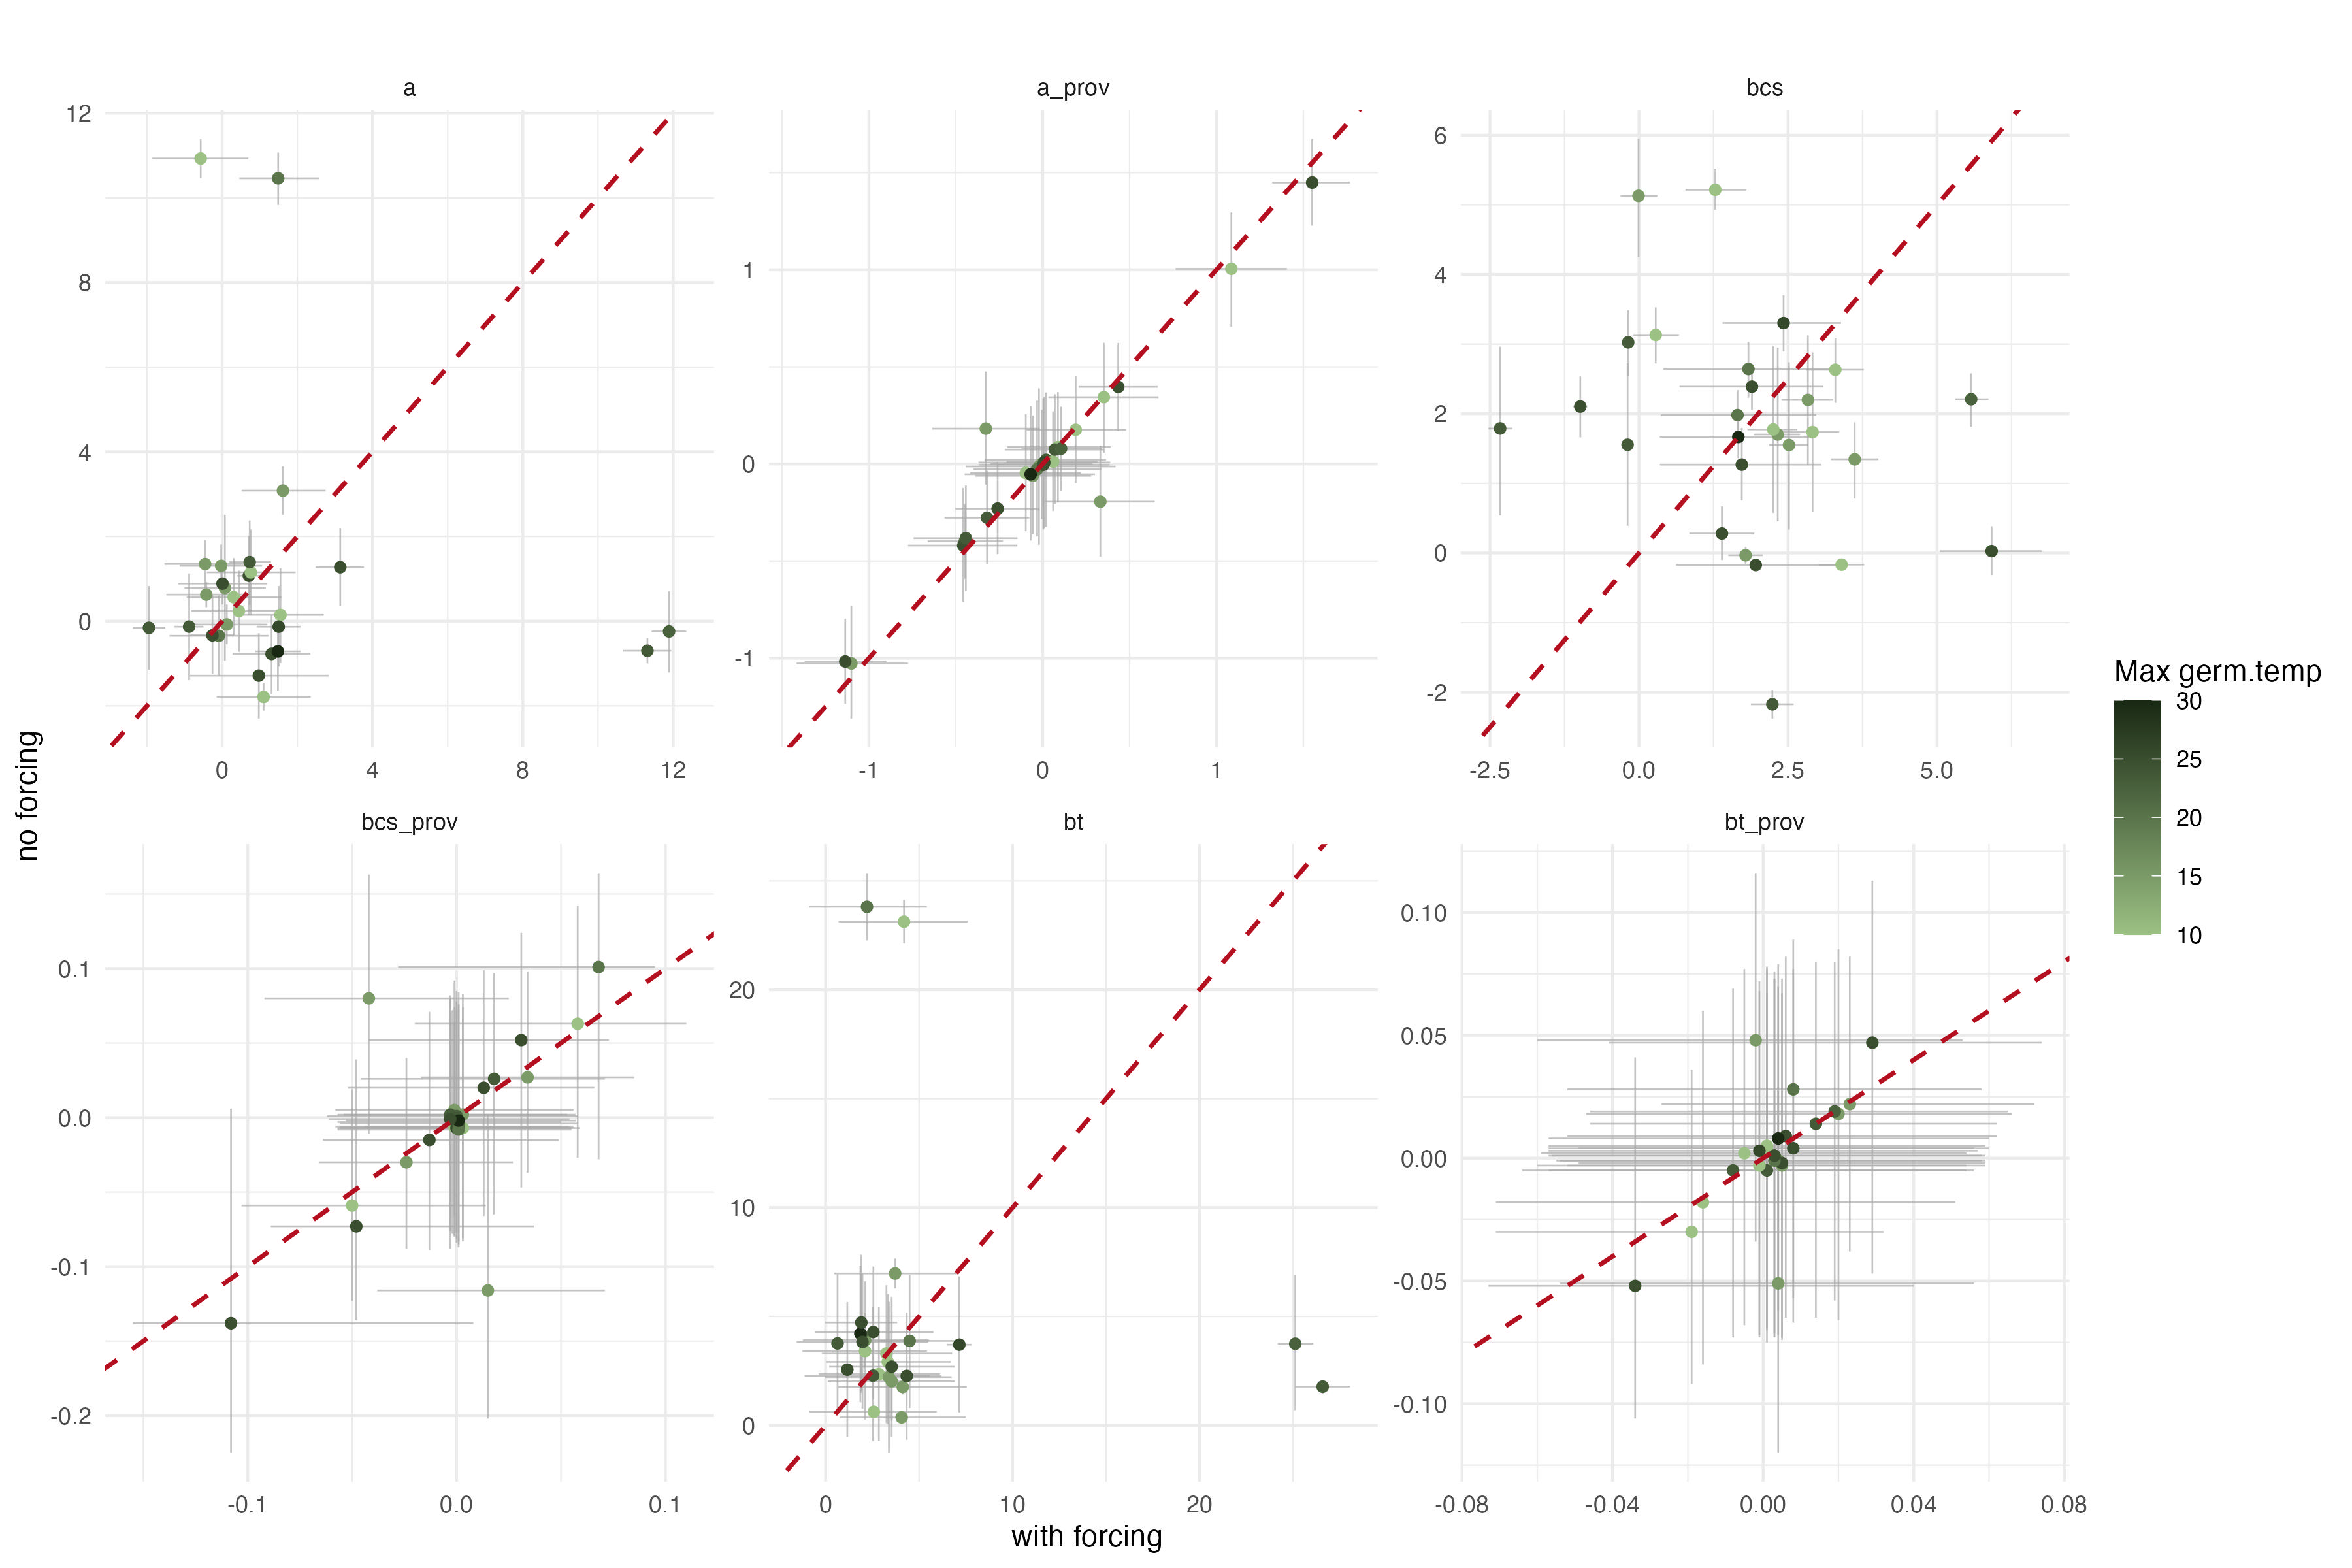
\includegraphics[width=0.7\textwidth]{../../analyses/analyseSeedCues/provenance/figures/forcingComparisonMaxGermtemp.jpeg}
\caption{Datasets with forcing vs no forcing color coded by max temperature} %emw11Aug: Showing what line? This is the annoying stuff you add now but WAY more annoying to try to figure it out later. For all the figures, explain the lines and the words (bcs etc.) or remove the words if you basically explain them elsewhere. Or per . Also I would start each caption with either 'comparing forcing and no-forcing models' or 'results' and you may also want: 'comparing models: model with forcing' ... be sure all the results with the model we decide to go with either come all FIRST or all SECOND, don't mix. 
\label{fig:maxGermTemp}
\end{figure}

% Number of unique germination treatments
\begin{figure}[!ht]
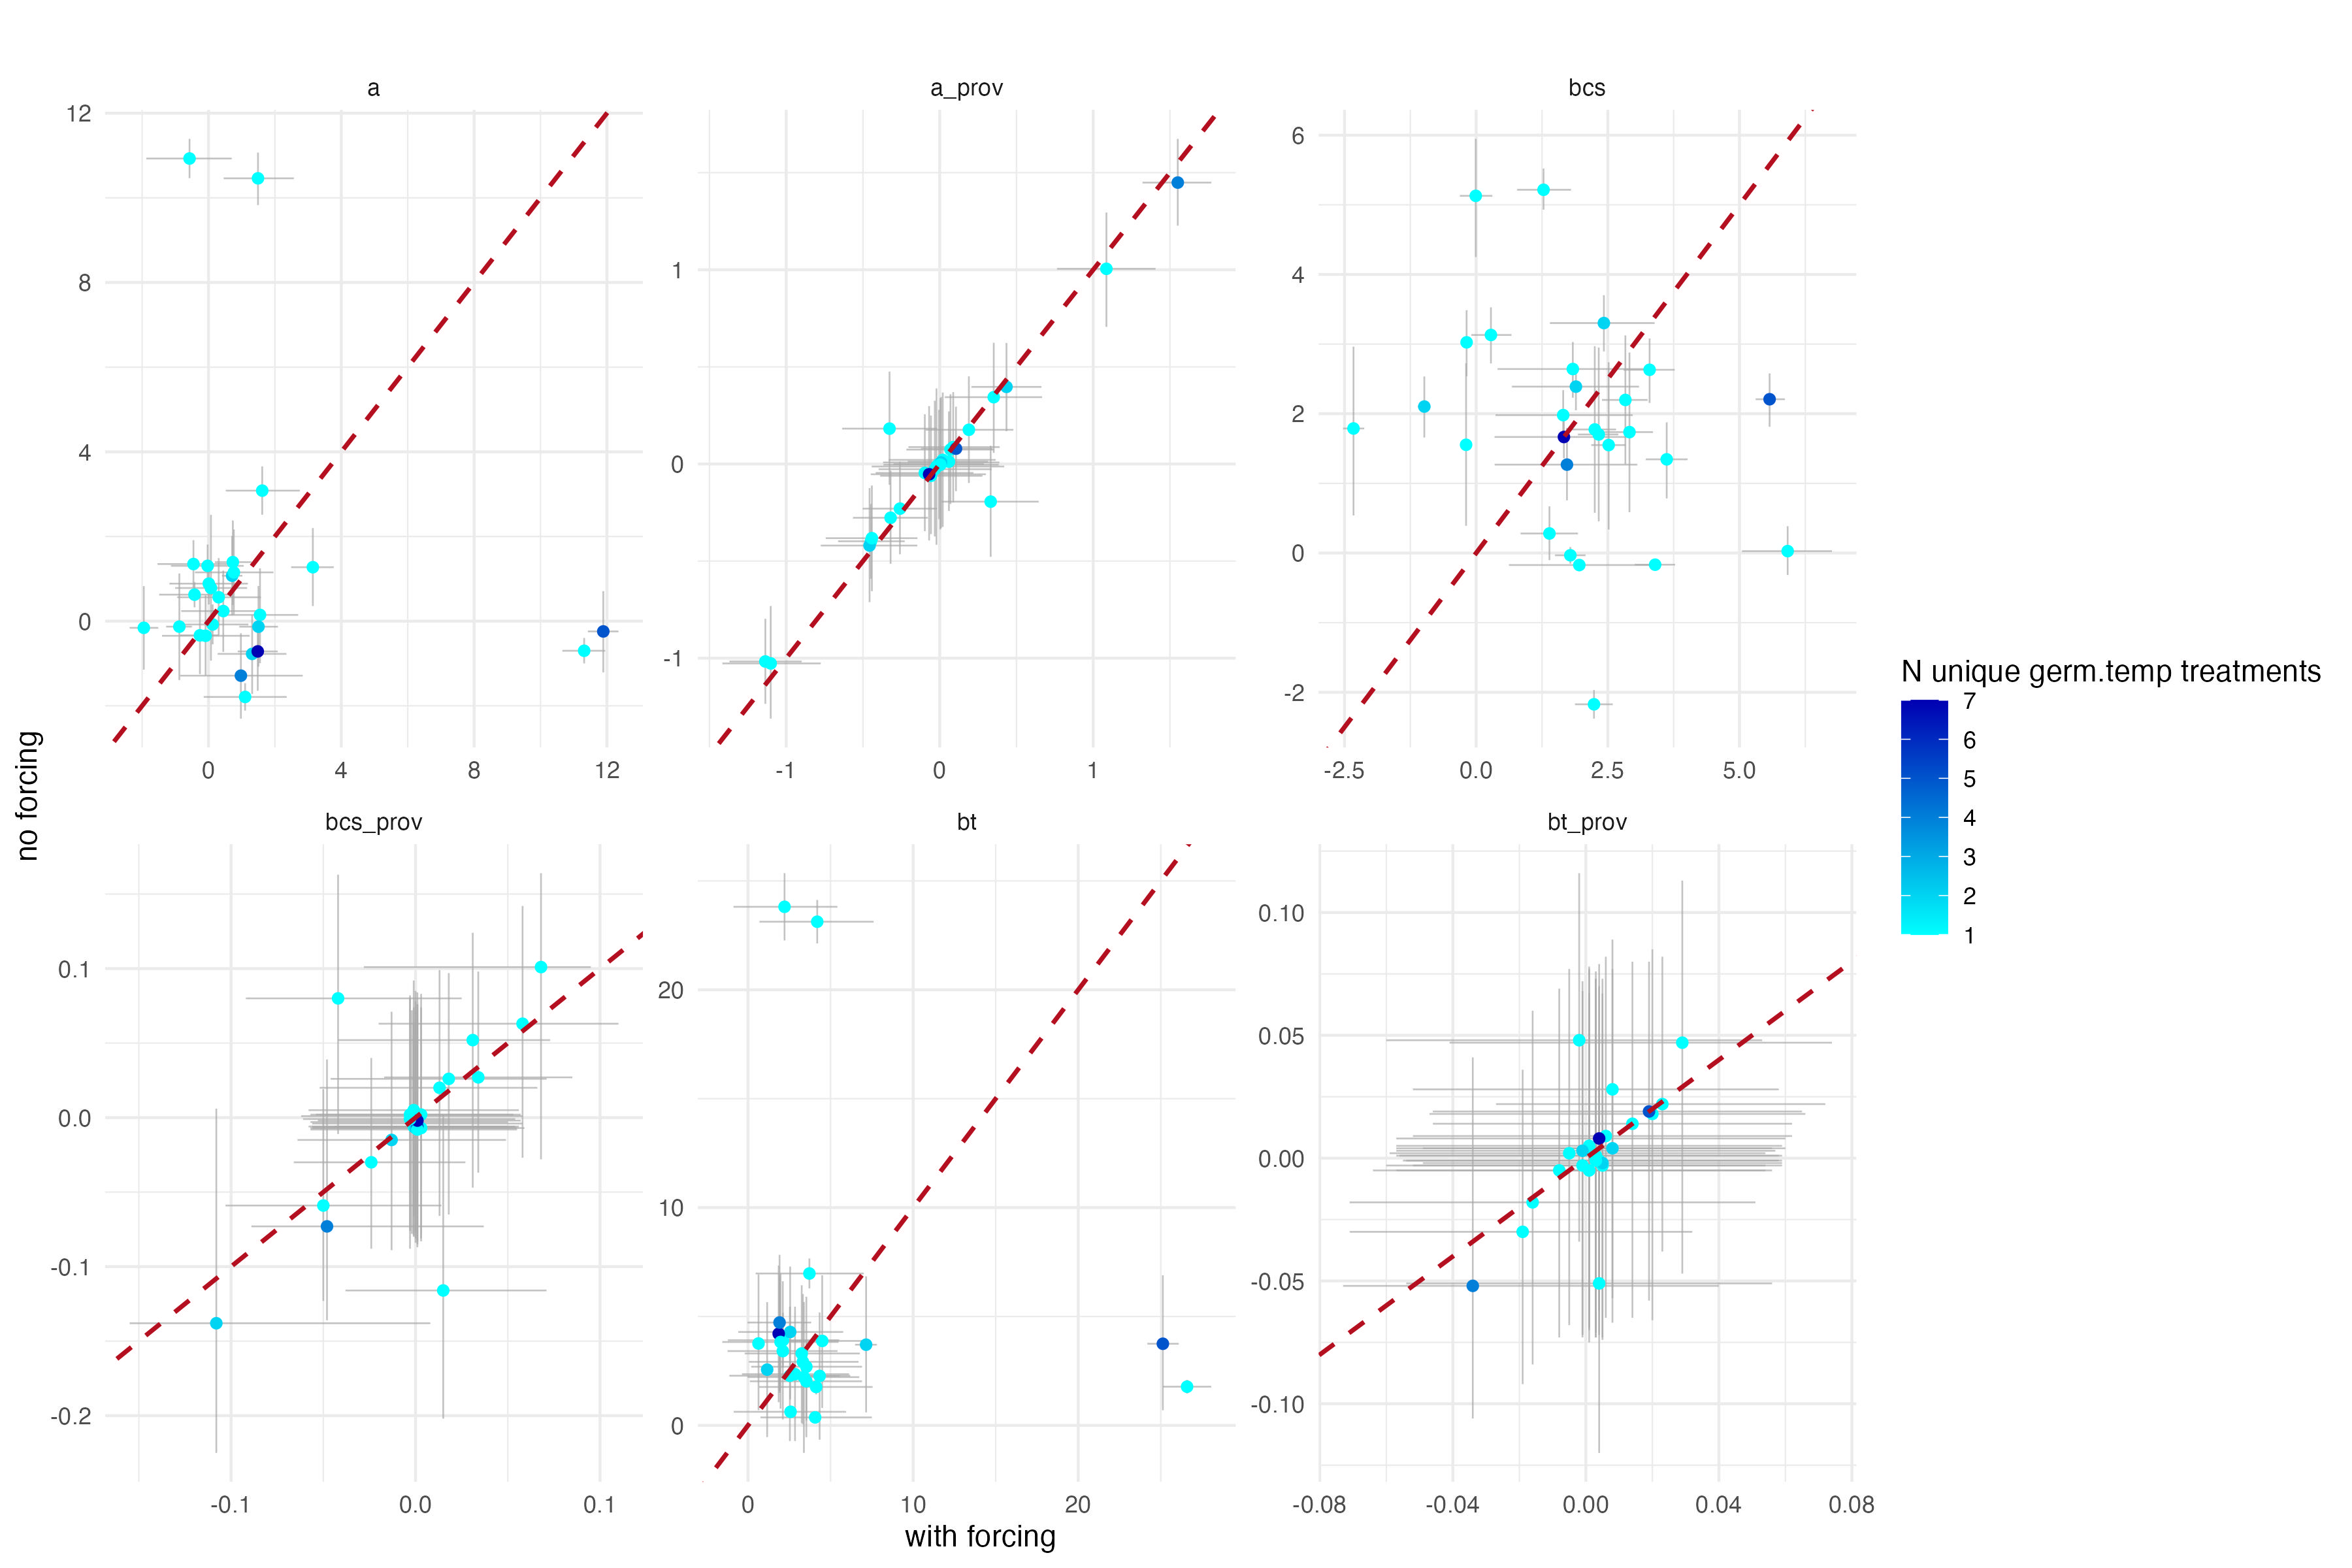
\includegraphics[width=0.7\textwidth]{../../analyses/analyseSeedCues/provenance/figures/forcingComparisonUniqueGermtemp.jpeg}
\caption{Datasets with forcing vs no forcing color coded by number of unique germ temp treatments}
\label{fig:uniqueGermTemp}
\end{figure}

% Germ temp interval
\begin{figure}[!ht]
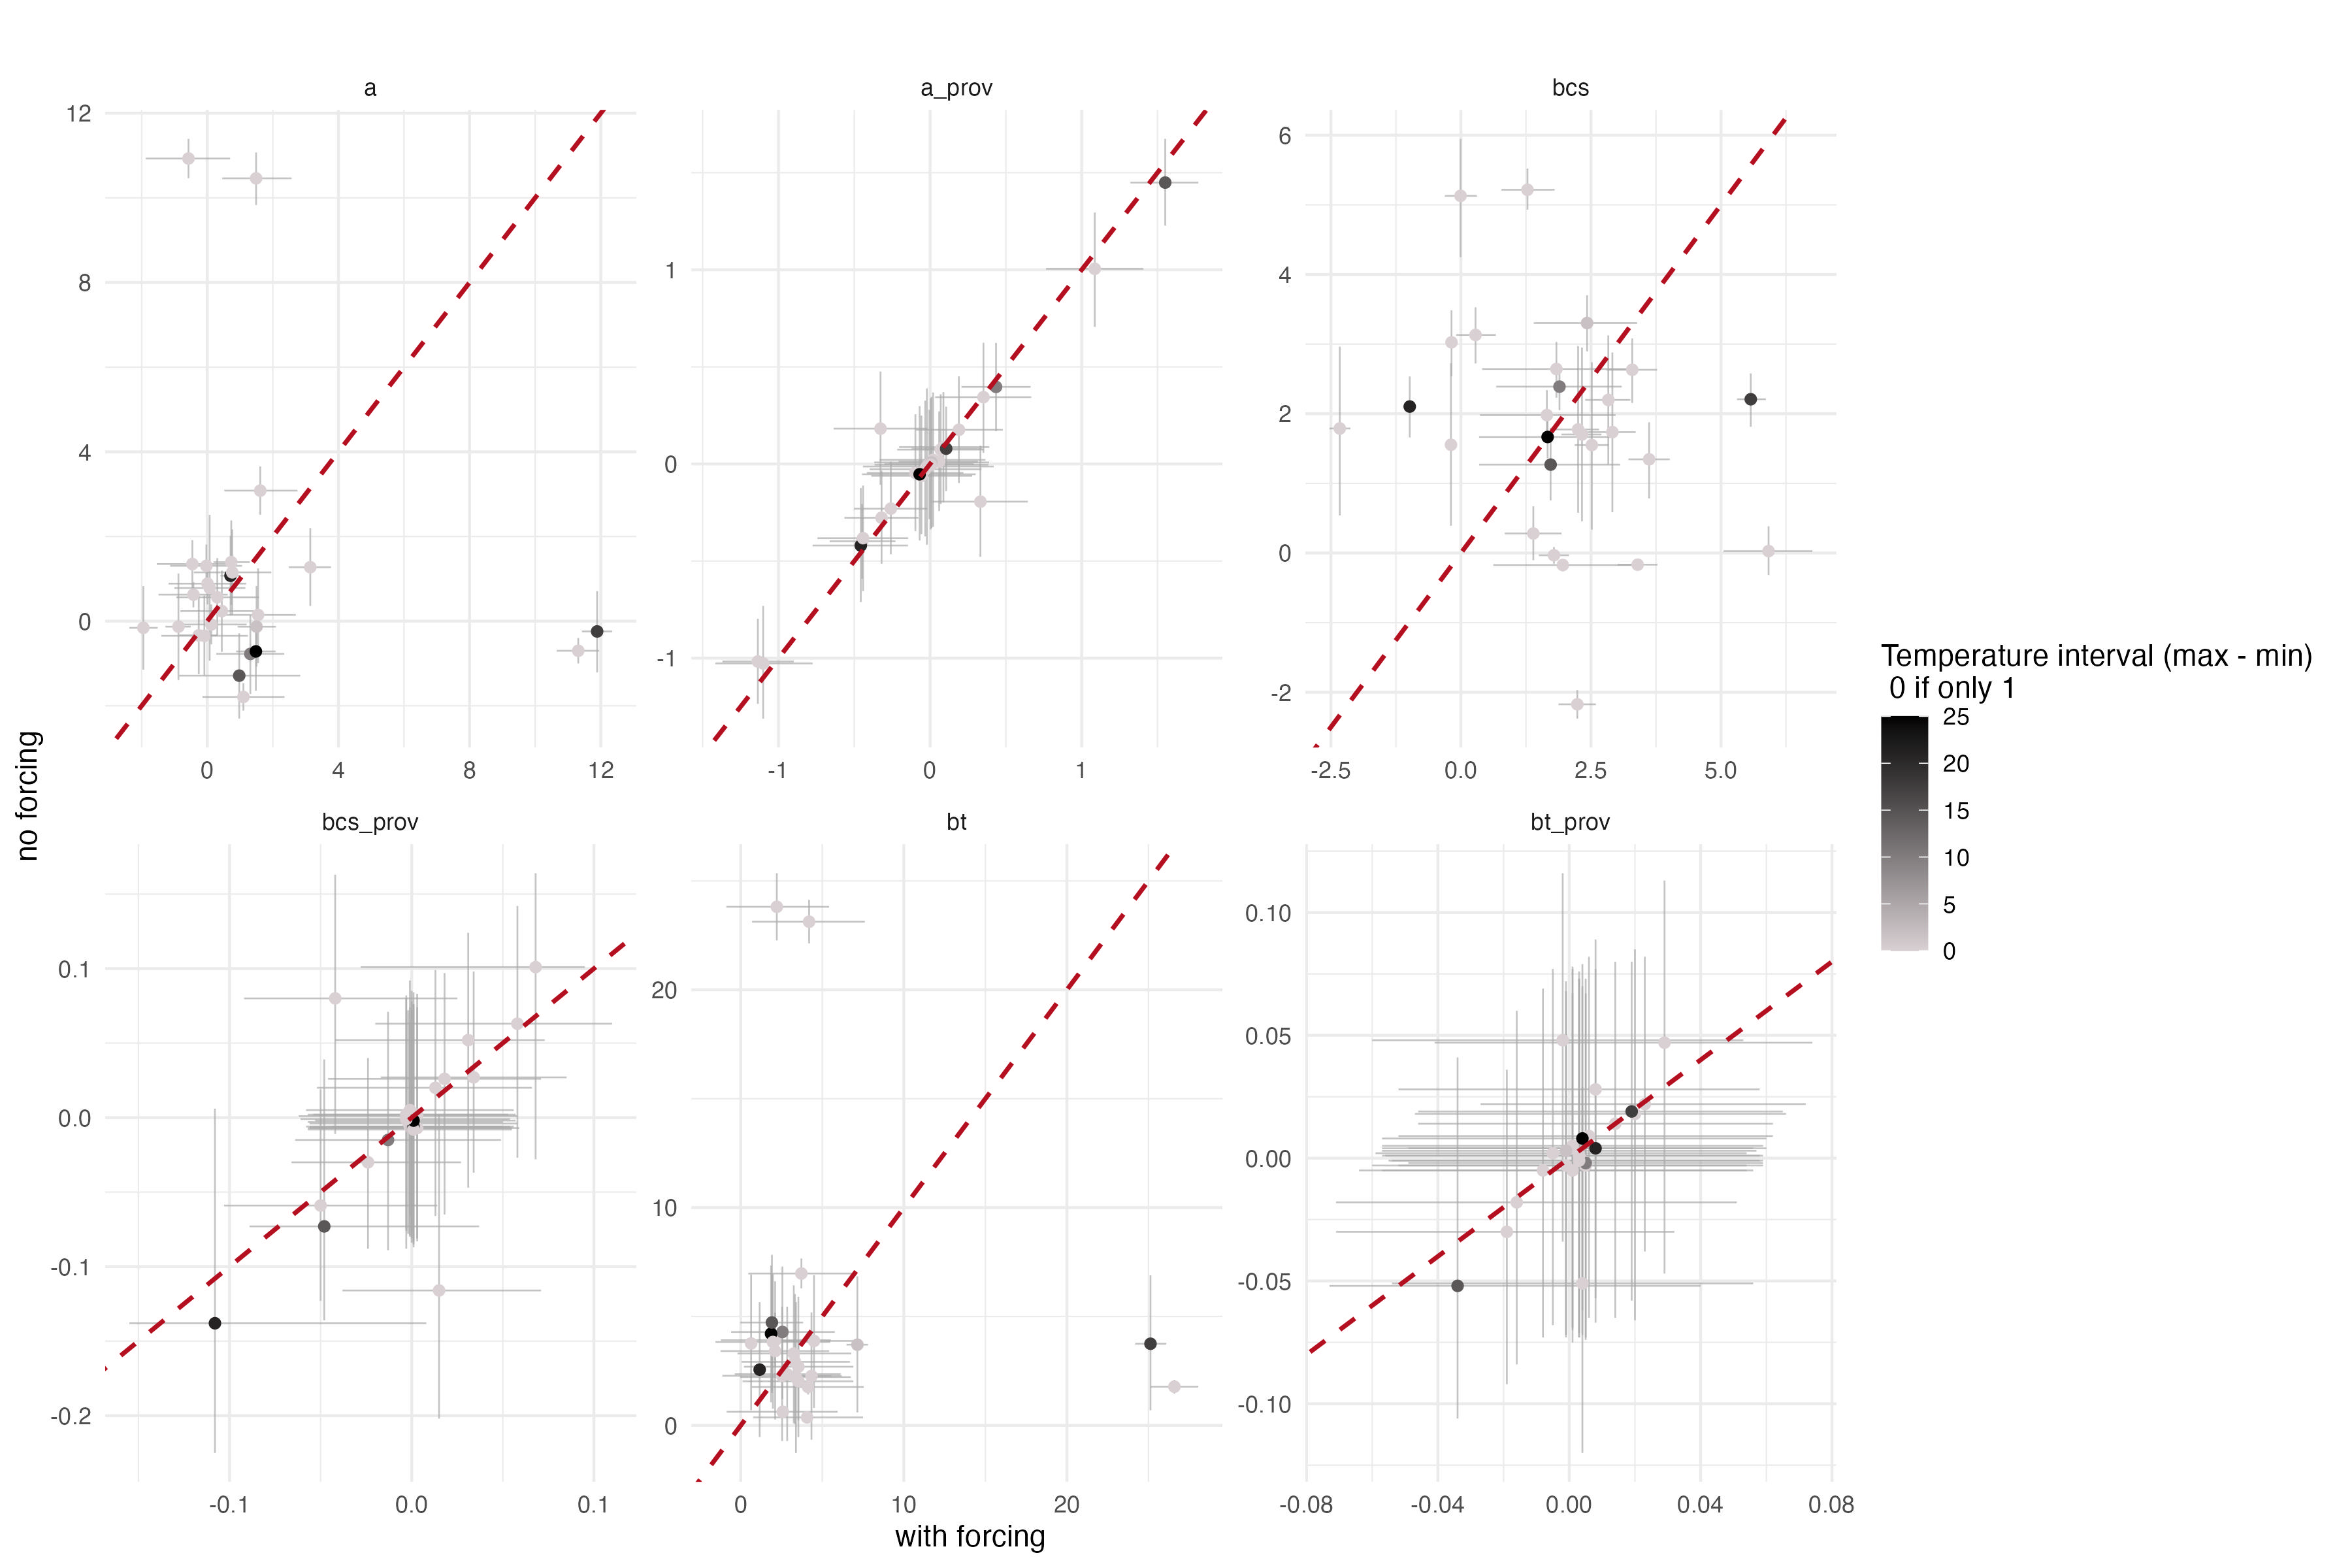
\includegraphics[width=0.7\textwidth]{../../analyses/analyseSeedCues/provenance/figures/forcingComparisonIntervGermtemp.jpeg}
\caption{Datasets with forcing vs no forcing color coded by the temperature interval in the study}
\label{fig:germTempInterval}
\end{figure}

\begin{figure}[!ht]
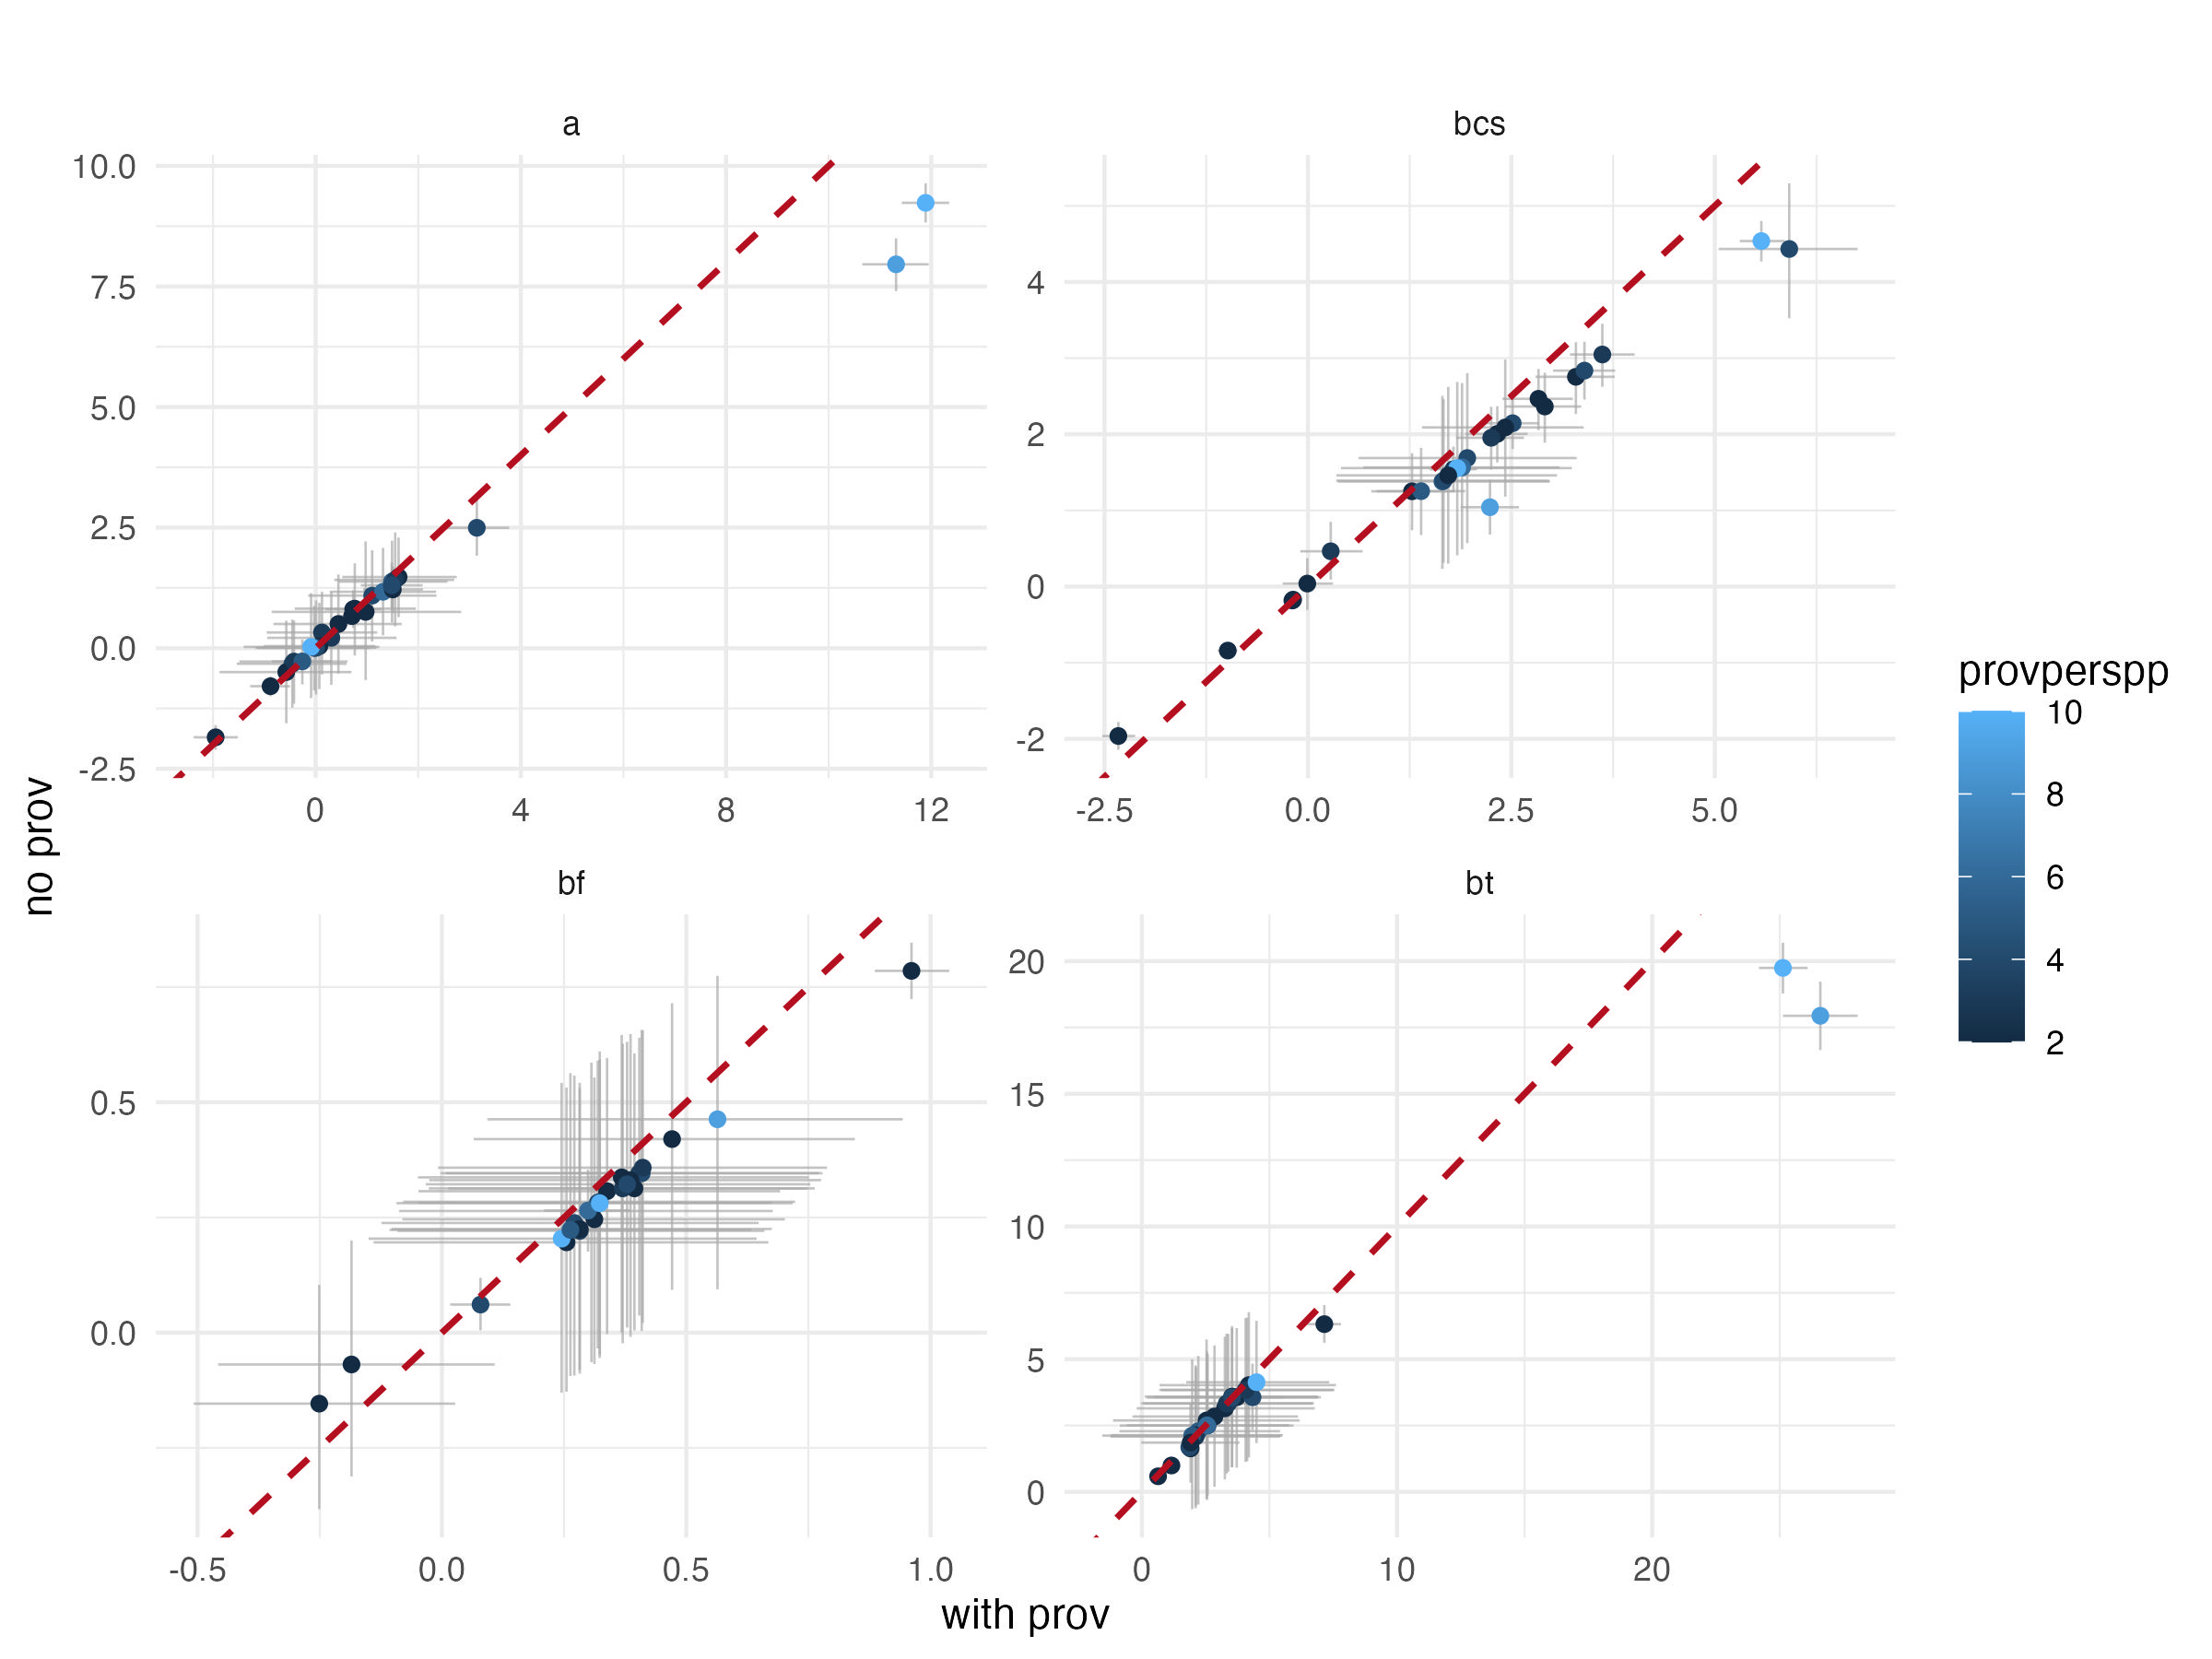
\includegraphics[width=0.7\textwidth]{../../analyses/analyseSeedCues/provenance/figures/11PlotProvNoProv.jpeg}
\caption{1:1 line plot to compare the model that includes provenance and excludes provenance.}
\label{fig:provNoProv}
\end{figure}



\begin{figure}[!ht]
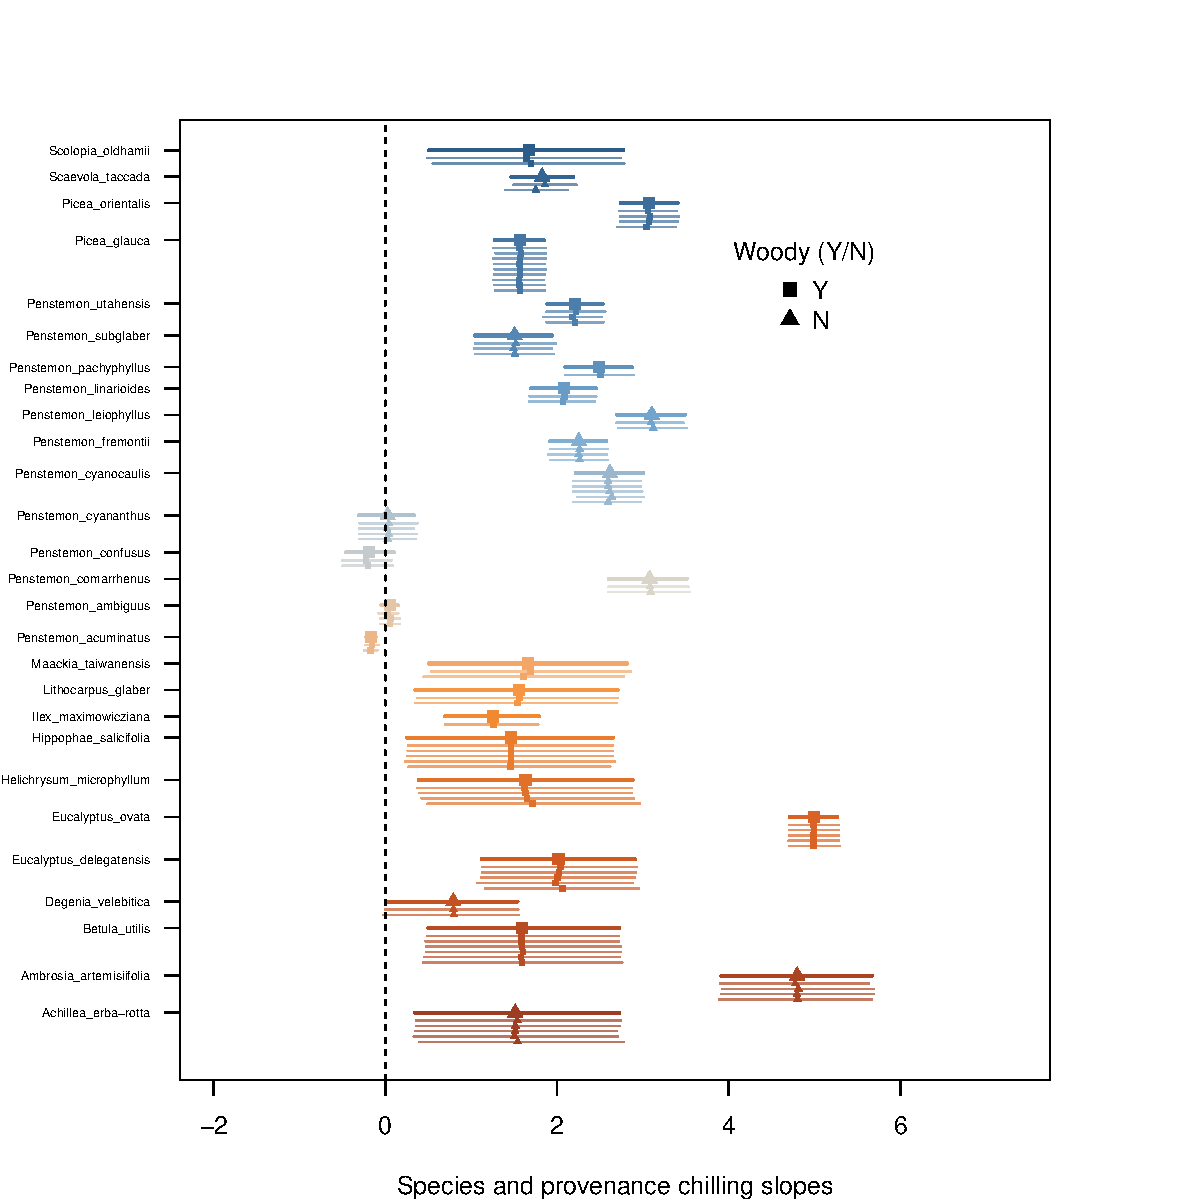
\includegraphics[width=0.7\textwidth]{../../analyses/analyseSeedCues/provenance/figures/muPlotProv_bcsprov.pdf}
\caption{Chilling slope parameters} %emw11Aug: What model? 
\label{fig:muChilling}
\end{figure}

\begin{figure}[!ht]
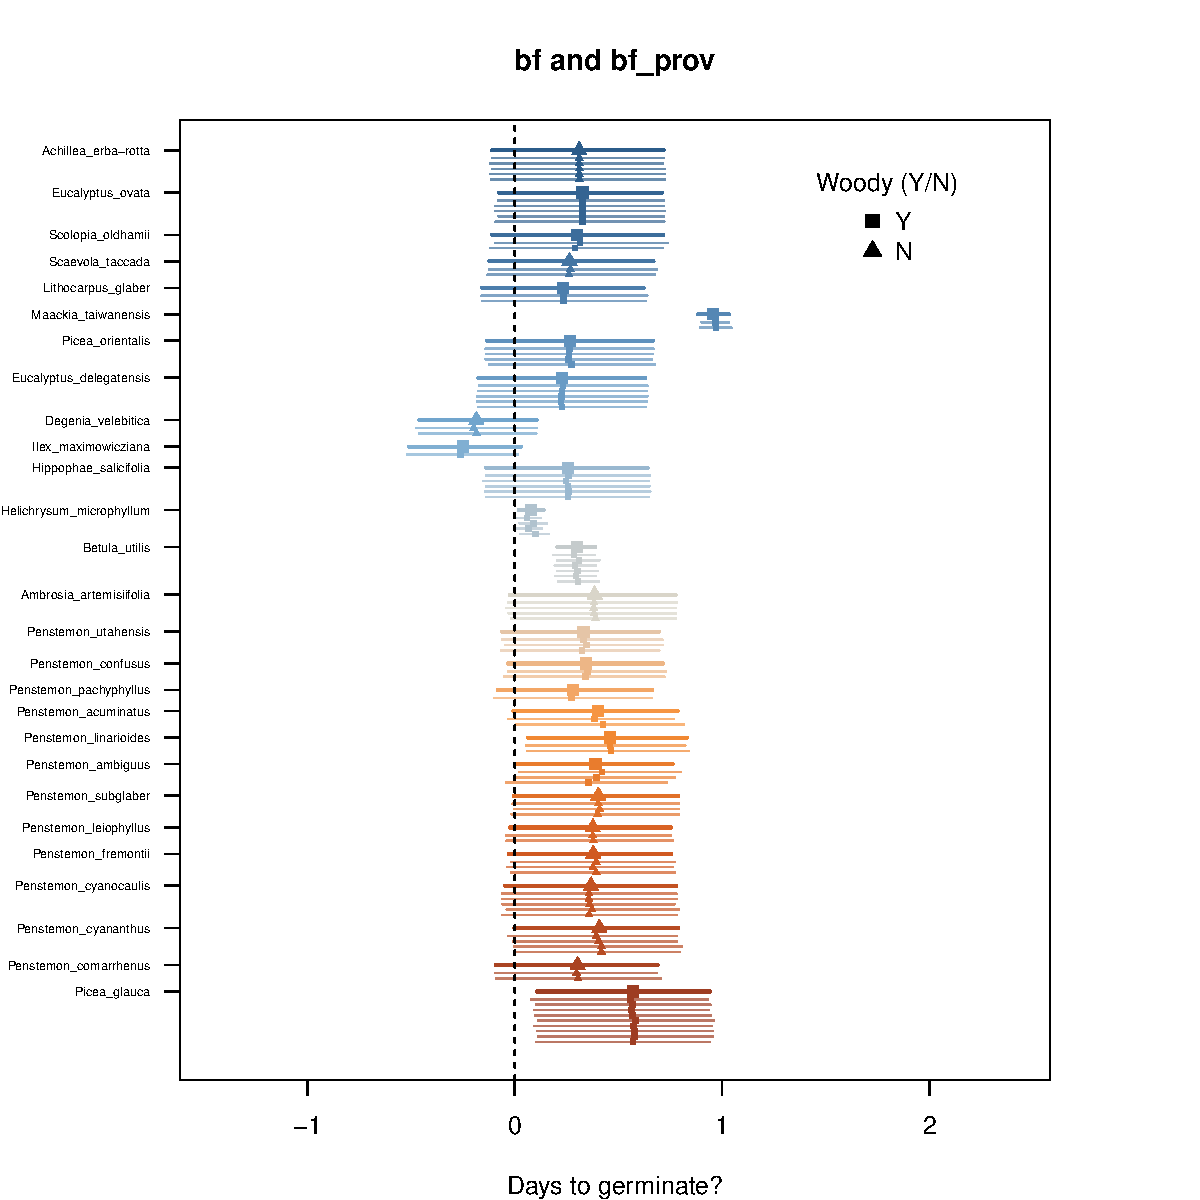
\includegraphics[width=0.7\textwidth]{../../analyses/analyseSeedCues/provenance/figures/muPlotProv_bfprov.pdf}
\caption{Forcing slope parameters} %emw11Aug: What model? 
\label{fig:muForcing}
\end{figure}

\begin{figure}[!ht]
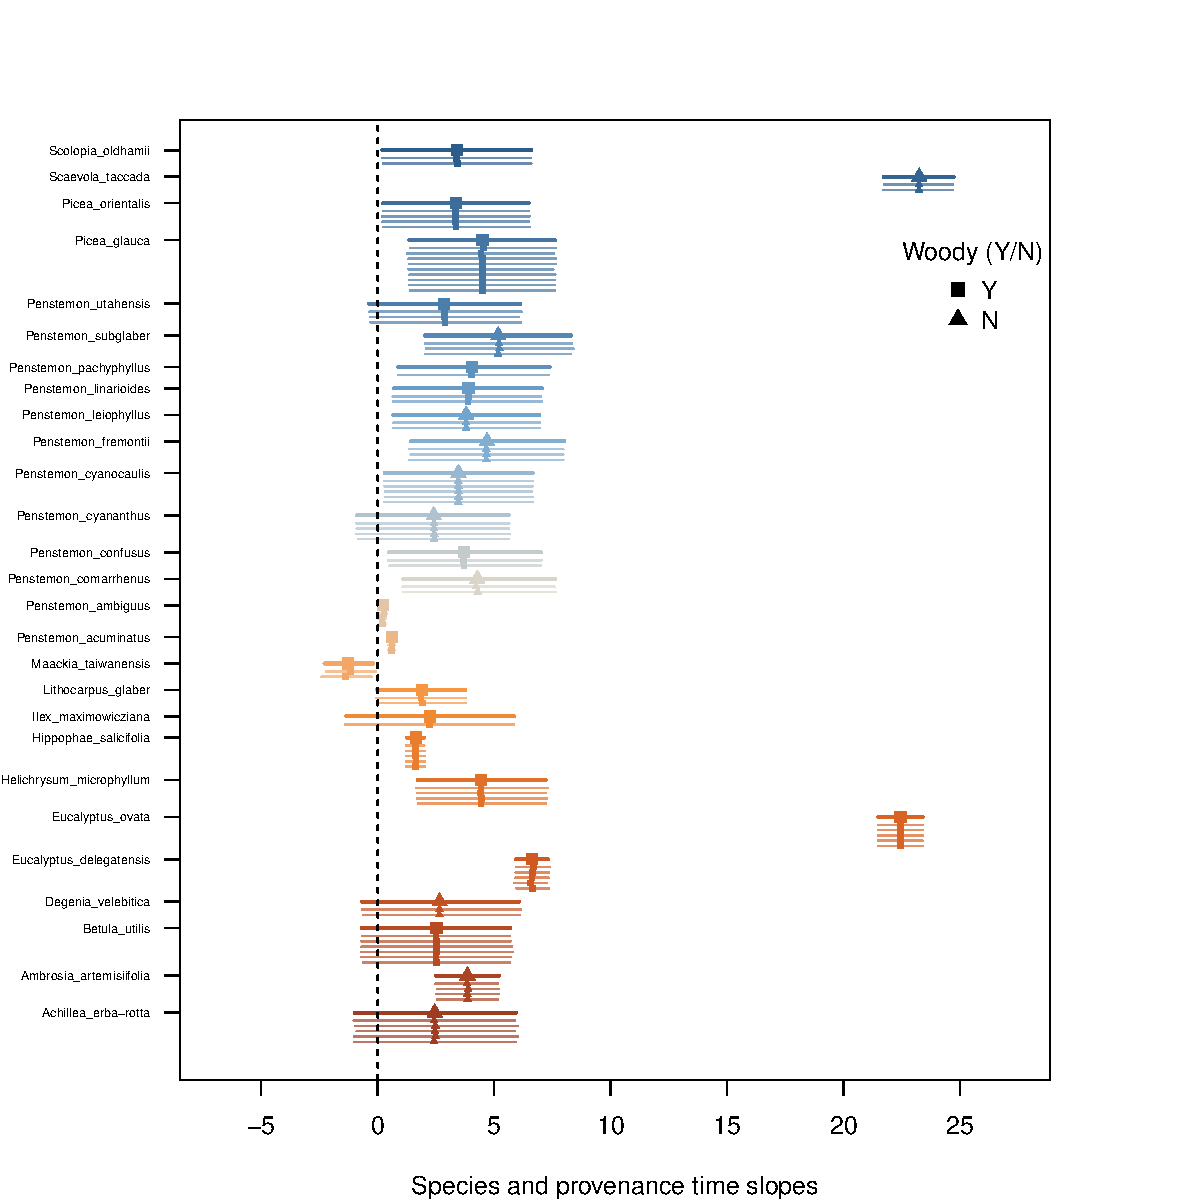
\includegraphics[width=0.7\textwidth]{../../analyses/analyseSeedCues/provenance/figures/muPlotProv_btprov.pdf}
\caption{Time slope parameters} %emw11Aug: What model? 
\label{fig:muTime}
\end{figure}

\begin{figure}[!ht]
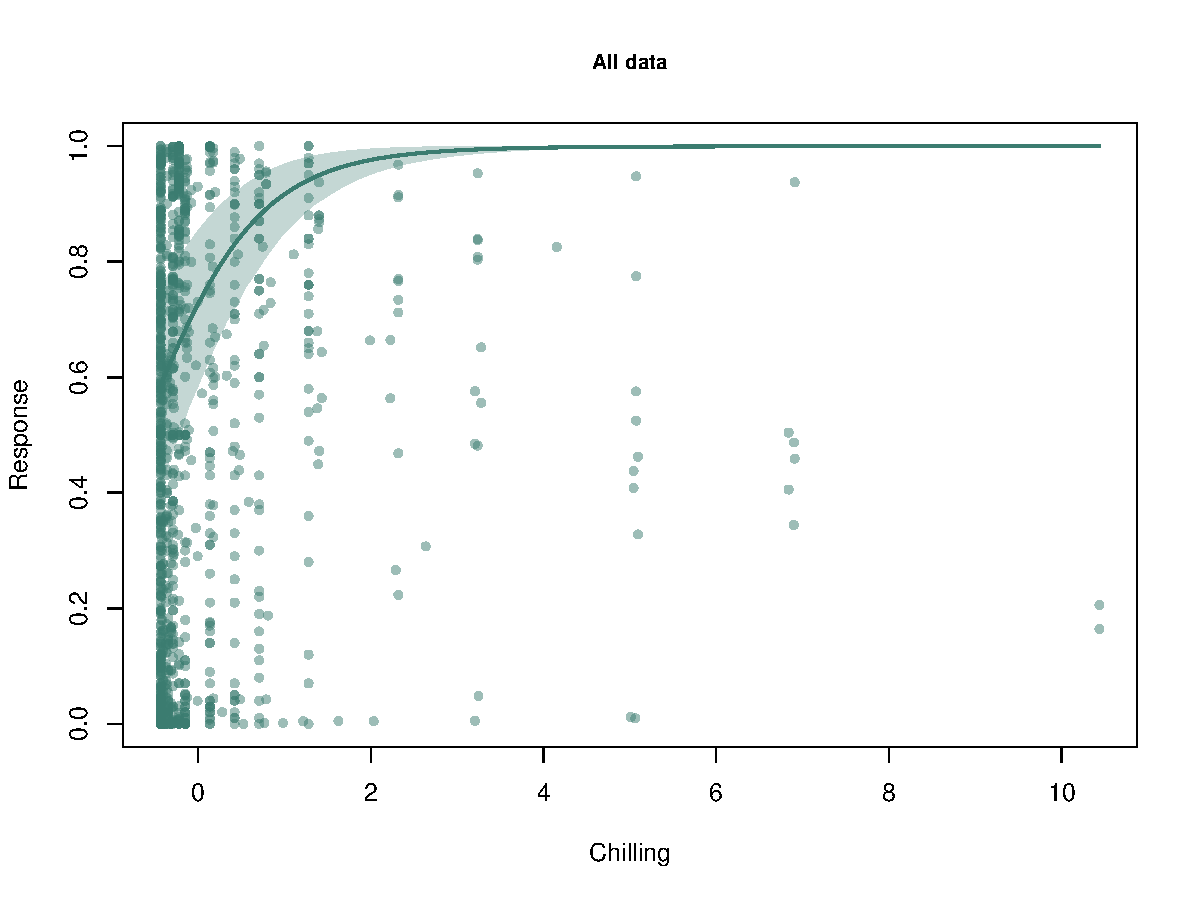
\includegraphics[width=0.7\textwidth]{../../analyses/analyseSeedCues/provenance/figures/retrodictiveChecks/PPC_meanT.pdf}
\caption{General response curve across all species as a function of chilling (scaled). We averaged the contribution of time and included it in the response curve.}
\label{fig:respCurveChilling} %emw11Aug: What model? 
\end{figure}


\begin{figure}[!ht]
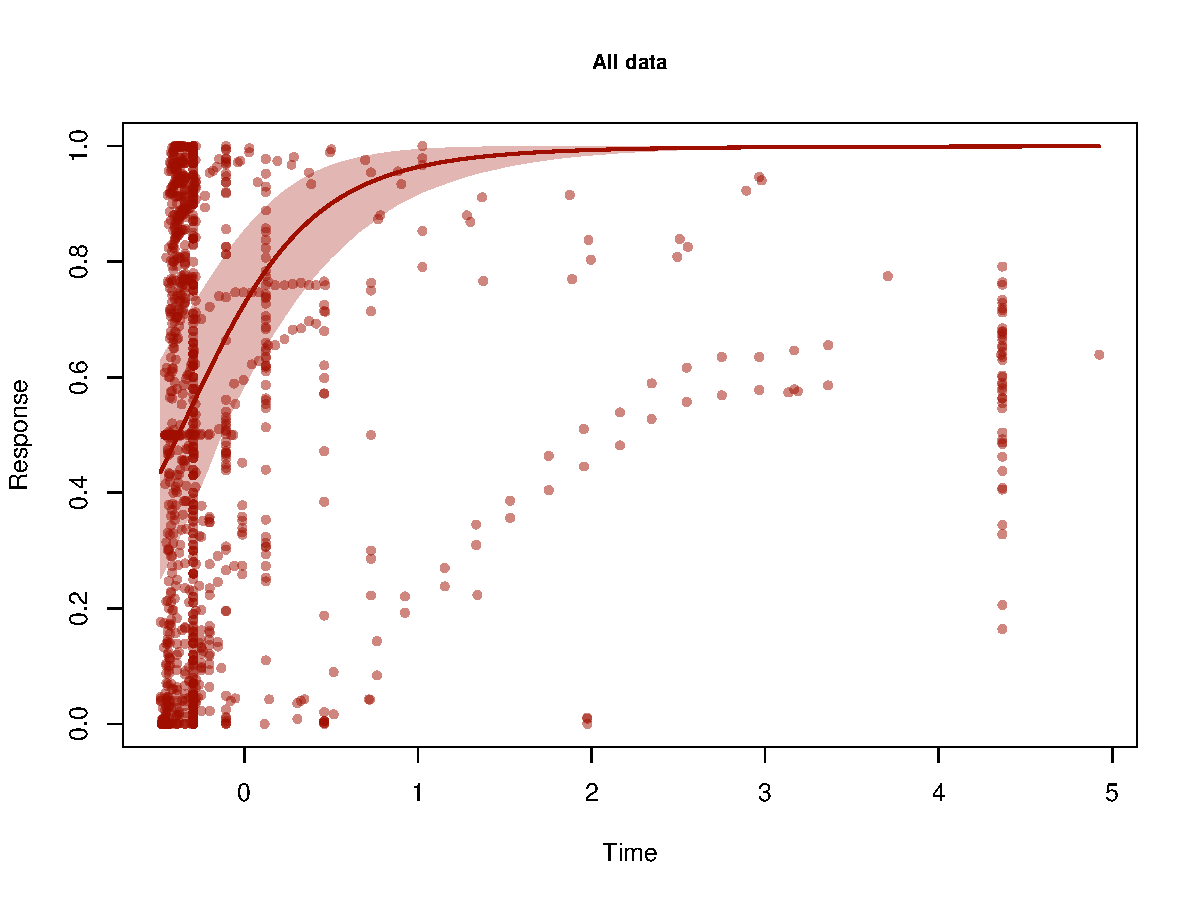
\includegraphics[width=0.7\textwidth]{../../analyses/analyseSeedCues/provenance/figures/retrodictiveChecks/PPC_meanC.pdf}
\caption{General response curve across all species as a function of time (scaled). We averaged the contribution of chilling and included it in the response curve.}
\label{fig:respCurveTime} %emw11Aug: What model? 
\end{figure}

\end{document}
